%%%%%%%%%%%%%%%%%%%%%%%%%%%%%%%%%%%%%%%%%
%
% (c) 2019 by Jennifer Laaser
%
% This work is licensed under the Creative Commons Attribution-NonCommercial-ShareAlike 4.0 International License. To view a copy of this license, visit http://creativecommons.org/licenses/by-nc-sa/4.0/ or send a letter to Creative Commons, PO Box 1866, Mountain View, CA 94042, USA.
%
% The current source for these materials is accessible on Github: https://github.com/jlaaser/pogil-polymers
%
%%%%%%%%%%%%%%%%%%%%%%%%%%%%%%%%%%%%%%%%%

\renewcommand{\figpath}{content/polymchem/networks/network-chaingrowth/figs}
\renewcommand{\labelbase}{network-chaingrowth}

\begin{activity}[Synthesis of Polymer Networks by Random Crosslinking]

\begin{instructornotes}
	This activity introduces students to concepts related to the synthesis of polymer networks by random crosslinking of pre-formed polymer chains and by chain-growth polymerization with a difunctional monomer.
	
	After completing this activity, students will be able to:
	\begin{enumerate}
		\item Identify the minimum number of monomers per chain that must be crosslinked to form a network
		\item Calculate the molecular weight between crosslinks in a crosslinked polymer network
		\item Calculate the amount of difunctional monomer necessary to form a crosslinked polymer network in a free-radical polymerization
	\end{enumerate}
	
	\subsection*{Activity summary:}
	\begin{itemize}
		\item \textbf{Activity type:} Learning Cycle
		\item \textbf{Content goals:} Synthesis of Polymer Networks
		\item \textbf{Process goals:} %https://pogil.org/uploads/attachments/cj54b5yts006cklx4hh758htf-process-skills-official-pogil-list-2015-original.pdf
			written communication, critical thinking, information processing
		\item \textbf{Duration:} TBD
		\item \textbf{Instructor preparation required:} none beyond knowledge of relevant content
		\item \textbf{Related textbook chapters:}
			\begin{itemize}
				\item \emph{Polymer Chemistry} (Hiemenz \& Lodge): section 10.1
			\end{itemize}
		%\item \textbf{Facilitation notes:}
		%	\begin{itemize}
		%		\item \dots
		%	\end{itemize}
	\end{itemize}
	
\end{instructornotes}


\begin{model}[Linking Polymer Strands]
	\label{\labelbase:mdl:linking}

	One way to synthesize a polymer network is to crosslink pre-formed polymer chains.
	
	Consider the following collection of polymer chains:
	
	\centerline{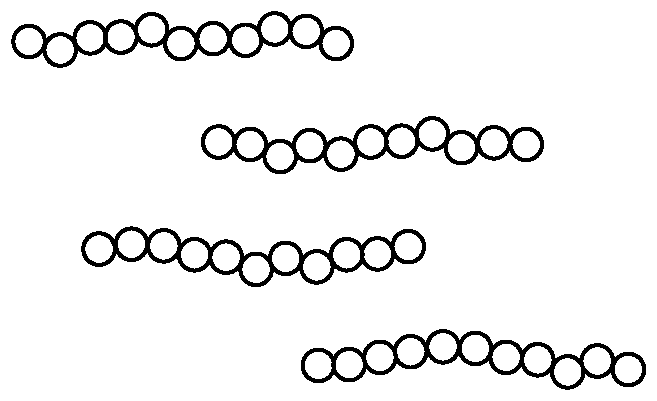
\includegraphics[width=0.5\textwidth]{\figpath/Model1_linking_blank.pdf}}
	
	To form a network, the chains must be crosslinked together to form a single large molecule:
	
	\centerline{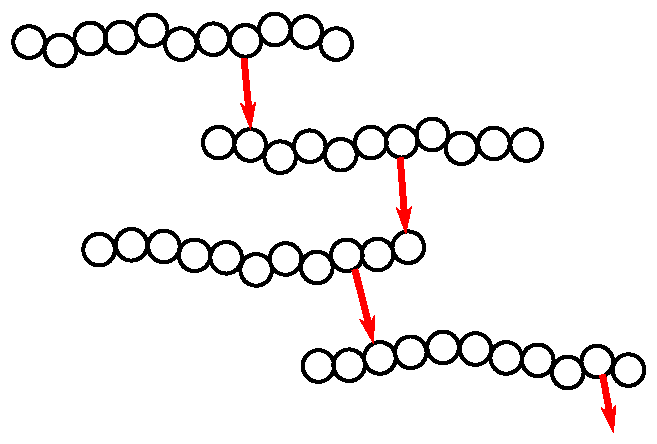
\includegraphics[width=0.5\textwidth]{\figpath/Model1_linking_arrows.pdf}}
	
	Here, we have drawn the crosslinks as arrows to make the analysis easier, but in practice, crosslinks do not have a specific orientation.
	
\end{model}


\begin{ctqs}

	\question In the picture shown in Model \ref{\labelbase:mdl:linking}, what is the \emph{minimum} number of ``outgoing'' crosslinks (arrows pointing away from the chain) that each polymer chain must have in order to allow a network to form?
	
		\begin{solution}[0.5in]
		
			one (each strand must link to the next to link all of the strands into a single molecule)
			
		\end{solution}
		
	\question If each polymer chain has $N$ monomers, what is the \emph{minimum fraction} of monomers, $x_c$, that must form an outgoing crosslink in order for a network to form?
	
		\begin{solution}[0.5in]
			$x_c = \frac{1}{N}$
		\end{solution}
		
	\question Briefly describe, in 2-3 complete sentences, how you could determine the minimum amount of crosslinker necessary to form a network from a polymer with molecular weight $M_n$.
	
		\begin{solution}[2in]
			First, take the molecular weight and divide by the monomer mass $M_0$ to find the degree of polymerization $N$.  Then, calculate the minimum fraction of monomers that need to be crosslinked to form a network using $x_c = \frac{1}{N_n}$.  Finally, use the total mass (or total number of moles) of monomer to calculate the total mass (or total number of moles) of crosslinker corresponding to this fraction.
		\end{solution}
		
	%\question get at the fact that it is weight-average molecular weight, not number-average molecular weight that matters
	
	%\question get at the calculation of molecular weight between crosslinks (this may need another model, with an appropriate image, or an adjustment to the image in Model 1...
\end{ctqs}

%\begin{model}[Chain-Growth Polymerization]

	% show chemistry of styrene + divinylbenzene - get students to realize that each difunctional monomer essentially forms an "outgoing" crosslink, and then connect minimum amount of crosslinker needed to the kinetic chain length
	
%\end{model}

%\begin{exercises}

%	\exercise Show the proposed chemistry of rubber vulcanization and give a problem about it
	
%\end{exercises}


%\begin{problems}
%
%	\problem First exercise
%	\problem Second exercise
%	
%\end{problems}


	
\end{activity}